\chapter{Phân tích và Thiết kế Hệ thống}
\label{chap:overview}

\section{Kỹ nghệ Yêu cầu}

Các yêu cầu hệ thống được thu thập từ quy trình hướng dẫn đồ án tốt nghiệp thực tế tại trường đại học và được cấu trúc hóa theo tiêu chuẩn IEEE Std 29148-2018~\cite{ieee29148} đối với đặc tả chức năng, cùng tiêu chuẩn ISO/IEC 25010:2023~\cite{iso25010} đối với các thuộc tính chất lượng sản phẩm phần mềm.

\subsection{Yêu cầu chức năng (FR)}

Mỗi Yêu cầu chức năng (FR) được đặc tả dưới dạng một nghĩa vụ nguyên tử, có thể kiểm thử độc lập, gắn với một tác nhân tường minh và mức độ ưu tiên rõ ràng (\textbf{Bắt buộc} [\textit{Must}] hoặc \textbf{Nên có} [\textit{Should}]). Bảng~\ref{tab:func-reqs} liệt kê mười sáu yêu cầu chức năng cốt lõi được phân nhóm theo năm phân hệ chức năng.

{\setlength{\tabcolsep}{3.5pt}
\begin{longtable}{|C{0.10}|L{0.15}|L{0.39}|C{0.11}|L{0.25}|}
\caption{Các yêu cầu chức năng nguyên tử được tổ chức theo từng phân hệ (IEEE 29148).}\label{tab:func-reqs}\\
\hline
\textbf{Mã} & \textbf{Tác nhân} & \textbf{Đặc tả yêu cầu} & \textbf{Ưu tiên} & \textbf{Tiêu chí nghiệm thu} \\
\hline
\endfirsthead
\multicolumn{5}{c}{\itshape Bảng \thetable\ (tiếp theo trang trước)}\\
\hline
\textbf{Mã} & \textbf{Tác nhân} & \textbf{Đặc tả yêu cầu} & \textbf{Ưu tiên} & \textbf{Tiêu chí nghiệm thu} \\
\hline
\endhead
\hline
\multicolumn{5}{r}{\itshape Xem tiếp trang sau}\\
\endfoot
\hline
\endlastfoot
\multicolumn{5}{|l|}{\textbf{Phân hệ 1: Định danh, Quản lý phiên đăng nhập và Kiểm soát truy cập}} \\
\hline
\textbf{\texttt{FR-01}} & Khách / Sinh viên & Hệ thống cho phép đăng ký tài khoản, xác thực mã kích hoạt email và mã đặt lại mật khẩu dùng một lần, đồng thời xác thực phiên làm việc qua thông tin đăng nhập nội bộ hoặc Google OAuth2. & \textbf{Bắt buộc} & Từ chối token sai/hết hạn; JWT đã thu hồi trả về \textbf{HTTP 401}. \\
\hline
\textbf{\texttt{FR-02}} & Mọi vai trò & Hệ thống thực thi kiểm soát truy cập dựa trên vai trò (\texttt{user}, \texttt{teacher}, \texttt{admin}), khóa API cá nhân và kiểm tra quyền sở hữu chéo giữa người dùng trên mọi tài nguyên. & \textbf{Bắt buộc} & Truy cập chéo bài nộp/kết luận của người khác trả về \textbf{HTTP 403} (0 lỗi IDOR). \\
\hline
\multicolumn{5}{|l|}{\textbf{Phân hệ 2: Tiếp nhận tài liệu, Phân tích cú pháp và Liên kết hai chiều}} \\
\hline
\textbf{\texttt{FR-03}} & Sinh viên / Giảng viên & Hệ thống tiếp nhận tải lên từng bản thảo hoặc theo lô ở định dạng PDF, DOCX, BibTeX và RIS sau khi kiểm tra byte định danh (magic bytes), dung lượng tệp, số trang và hạn mức tháng. & \textbf{Bắt buộc} & Từ chối gọn các tệp giả mạo PDF/DOCX hoặc vượt hạn mức tải lên. \\
\hline
\textbf{\texttt{FR-04}} & Sinh viên / Giảng viên & Hệ thống phát trực tiếp tiến độ thời gian thực qua tám giai đoạn xử lý và tự động hoàn lại hạn mức tải lên nếu tác vụ bất đồng bộ thất bại vĩnh viễn. & \textbf{Bắt buộc} & SSE phát đủ các bước 0--7; tác vụ lỗi hoàn hạn mức nguyên tử. \\
\hline
\textbf{\texttt{FR-05}} & Pipeline & Hệ thống phân tách bản thảo tải lên thành văn bản chính, các dấu trích dẫn trong bài kèm ngữ cảnh xung quanh và danh mục tài liệu tham khảo trên 12 chuẩn trích dẫn (bao gồm văn bản pháp luật Việt Nam). & \textbf{Bắt buộc} & Phát hiện danh mục tài liệu đạt \textbf{$\ge 97\%$} trên bộ kiểm thử 310 PDF đa chuẩn. \\
\hline
\textbf{\texttt{FR-06}} & Pipeline & Hệ thống phát hiện tệp PDF bản quét (scan) hoặc PDF tiếng Việt dùng bảng mã cũ để kích hoạt nhận dạng ký tự quang học (OCR) có chọn lọc hoặc chuẩn hóa bảng mã. & Nên có & Các trang quét được ghi nhận đầy đủ trong siêu dữ liệu chẩn đoán tài liệu. \\
\hline
\textbf{\texttt{FR-07}} & Pipeline & Hệ thống liên kết từng dấu trích dẫn trong bài tới mục tài liệu tham khảo đích và phân loại mỗi cạnh liên kết vào một trong tám trạng thái ánh xạ cấu trúc. & \textbf{Bắt buộc} & Cô lập chính xác trích dẫn mồ côi, tài liệu không được trích dẫn và lệch năm. \\
\hline
\multicolumn{5}{|l|}{\textbf{Phân hệ 3: Truy xuất liên hợp và Xác thực định danh}} \\
\hline
\textbf{\texttt{FR-08}} & Pipeline & Hệ thống truy vấn kho học thuật ngoại tuyến và các cơ sở dữ liệu trực tuyến theo lĩnh vực, đồng thời ghi nhận nguồn gốc thành công, thất bại và giới hạn tần suất (rate limit) của từng nguồn. & \textbf{Bắt buộc} & Độ phủ ngoại tuyến \textbf{$\ge 99\%$}; phân biệt rõ lỗi \textbf{HTTP 429} với 0 kết quả. \\
\hline
\textbf{\texttt{FR-09}} & Pipeline & Hệ thống xác thực các URL và DOI được trích dẫn thông qua truy vấn HTTP chống SSRF, siêu dữ liệu Retraction Watch và bản lưu Internet Archive. & \textbf{Bắt buộc} & Chặn các địa chỉ IP nội bộ; gắn cờ \textbf{$100\%$} công trình đã bị rút bài. \\
\hline
\multicolumn{5}{|l|}{\textbf{Phân hệ 4: Kiểm chứng thần kinh -- biểu trưng, Chấm điểm và Khắc phục lỗi}} \\
\hline
\textbf{\texttt{FR-10}} & Pipeline & Hệ thống tính toán độ tương đồng từ vựng, ngữ nghĩa và xuyên ngôn ngữ (\texttt{VI}$\leftrightarrow$\texttt{EN}) giữa nhận định trong bài với tiêu đề/tóm tắt của tài liệu nguồn truy xuất được. & \textbf{Bắt buộc} & Nhận định mâu thuẫn và khớp xuyên ngôn ngữ được chấm điểm trong $[0,1]$. \\
\hline
\textbf{\texttt{FR-11}} & Pipeline & Hệ thống gán một trong năm nhãn kết luận, xác suất đã hiệu chuẩn Platt và danh sách có thứ tự các mã luật biểu trưng được kích hoạt cho từng tài liệu tham khảo. & \textbf{Bắt buộc} & Độ chính xác kiểm thử \textbf{$\ge 98.5\%$}, \textbf{$\text{ECE} \le 0.05$}, \textbf{$100\%$} vết luật. \\
\hline
\textbf{\texttt{FR-12}} & Pipeline & Hệ thống tính toán Điểm toàn vẹn trích dẫn (CIS) gồm năm thành phần trong đoạn $[0, 100]$ và sinh lời giải thích song ngữ (\texttt{EN}/\texttt{VI}). & \textbf{Bắt buộc} & Tổng trọng số thành phần bằng $1.00$; lời giải thích hiển thị cả EN \& VI. \\
\hline
\textbf{\texttt{FR-13}} & Sinh viên / Giảng viên & Hệ thống xuất báo cáo đã làm sạch an toàn (PDF, DOCX, CSV, JSON) và sinh danh mục tài liệu tham khảo đã sửa lỗi theo chuẩn APA, IEEE, TDTU, BibTeX, RIS và DOCX. & Nên có & Mục tài liệu sau sửa phản ánh đúng siêu dữ liệu chuẩn, không chứa macro. \\
\hline
\textbf{\texttt{FR-14}} & Sinh viên / Công khai & Hệ thống cấp liên kết chia sẻ ký mật mã có thời hạn kèm mã QR biên nhận xác thực để bên thứ ba tra cứu ở chế độ chỉ đọc. & Nên có & Token chia sẻ hết hạn hoặc bị chỉnh sửa trả về \textbf{HTTP 404/403}. \\
\hline
\multicolumn{5}{|l|}{\textbf{Phân hệ 5: Giám sát lớp học phần và Quản trị nền tảng}} \\
\hline
\textbf{\texttt{FR-15}} & Giảng viên & Hệ thống cho phép giảng viên quản lý lớp học qua mã tham gia, theo dõi thống kê toàn lớp cùng các trích dẫn ảo trùng lặp và ghi đè kết luận khi được cấp quyền. & \textbf{Bắt buộc} & Ghi đè cập nhật kết luận, tính lại CIS và ghi nhật ký kiểm toán. \\
\hline
\textbf{\texttt{FR-16}} & Quản trị viên & Hệ thống cho phép quản trị viên quản lý tài khoản, mã khuyến mãi, trạng thái bộ nhớ đệm, bộ ngắt mạch (circuit breaker) của nguồn ngoài và nhật ký kiểm toán. & \textbf{Bắt buộc} & Đặt lại bộ ngắt mạch và xóa bộ nhớ đệm có hiệu lực ngay lập tức. \\
\hline
\end{longtable}
}

\subsection{Yêu cầu phi chức năng (NFR)}

Nhằm đảm bảo khả năng vận hành thực tế trên hạ tầng phần cứng tiêu chuẩn của trường đại học không trang bị GPU, mười Yêu cầu phi chức năng (NFR) định lượng được ánh xạ vào các nhóm chất lượng theo chuẩn ISO/IEC 25010:2023 trong Bảng~\ref{tab:nfr-reqs}.

{\setlength{\tabcolsep}{3.5pt}
\begin{longtable}{|C{0.11}|L{0.25}|L{0.40}|L{0.24}|}
\caption{Các yêu cầu phi chức năng định lượng ánh xạ theo chuẩn ISO/IEC 25010:2023.}\label{tab:nfr-reqs}\\
\hline
\textbf{Mã} & \textbf{Thuộc tính ISO/IEC 25010} & \textbf{Yêu cầu chất lượng} & \textbf{Chỉ số mục tiêu / SLA} \\
\hline
\endfirsthead
\multicolumn{4}{c}{\itshape Bảng \thetable\ (tiếp theo trang trước)}\\
\hline
\textbf{Mã} & \textbf{Thuộc tính ISO/IEC 25010} & \textbf{Yêu cầu chất lượng} & \textbf{Chỉ số mục tiêu / SLA} \\
\hline
\endhead
\hline
\multicolumn{4}{r}{\itshape Xem tiếp trang sau}\\
\endfoot
\hline
\endlastfoot
\textbf{\texttt{NFR-01}} & \textbf{Hiệu quả hiệu năng} (Đặc tính thời gian) & Độ trễ kiểm chứng khi ấm bộ nhớ đệm (warm cache) đối với báo cáo đồ án 50 trang ($\sim$32 tài liệu tham khảo) trên phần cứng CPU. & \textbf{$P_{90} \le 2.5\text{\,s}$} (mạng diện rộng [WAN] lạnh $\le 15\text{\,s}$). \\
\hline
\textbf{\texttt{NFR-02}} & \textbf{Hiệu quả hiệu năng} (Sử dụng tài nguyên) & Mức chiếm dụng bộ nhớ thực (RSS) cực đại của tiến trình Python phía máy chủ khi phân tích chuyên khảo dài 150 trang. & \textbf{$\text{RSS} \le 1.5\text{\,GB}$}; độ tăng heap $\Delta \le 25\text{\,MB}$. \\
\hline
\textbf{\texttt{NFR-03}} & \textbf{Hiệu quả hiệu năng} (Dung lượng tải) & Xử lý các lượt tải lên đồng thời vào sát hạn nộp bài của lớp học mà không phát sinh lỗi khóa SQLite hoặc phản hồi HTTP 5xx. & \textbf{$50$ lượt tải lên đồng thời, $0\%$ lỗi}. \\
\hline
\textbf{\texttt{NFR-04}} & \textbf{Độ tin cậy} (Khả năng chịu lỗi) & Suy giảm nhẹ nhàng (graceful degradation) khi GROBID hoặc các API học thuật bên ngoài quá thời gian chờ hoặc trả về lỗi HTTP 429. & Tự động chuyển sang PyMuPDF dự phòng; \textbf{$100\%$ tạm hoãn an toàn} khi gặp 429. \\
\hline
\textbf{\texttt{NFR-05}} & \textbf{Tính phù hợp chức năng} & Không kết luận nhầm công trình hợp lệ là trích dẫn ảo và đảm bảo xác suất độ tin cậy được hiệu chuẩn tốt. & Báo nhầm trích dẫn ảo \textbf{$\le 0.1\%$}; \textbf{$\text{ECE} \le 0.05$}. \\
\hline
\textbf{\texttt{NFR-06}} & \textbf{Tính bảo mật} (Tính bí mật \& Toàn vẹn) & Bảo vệ chống tấn công SSRF, IDOR, chèn mã kịch bản chéo trang (XSS), chèn công thức CSV và dò mật khẩu vét cạn (brute-force). & \textbf{Chặn SSRF ghim IP}; băm \texttt{bcrypt} kèm muối + token SHA-256/\allowbreak HMAC. \\
\hline
\textbf{\texttt{NFR-07}} & \textbf{Khả năng tương tác} (Tính khả dụng) & Giao diện biên tập hỗ trợ chế độ Sáng và Tối dễ tiếp cận, hiển thị thông tin theo tầng (progressive disclosure) và bản địa hóa song ngữ. & Chuẩn \textbf{WCAG 2.1 AA} (tương phản $\ge 4.5:1$); $0\text{\,px}$ tràn lề. \\
\hline
\textbf{\texttt{NFR-08}} & \textbf{Hiệu quả hiệu năng} (Thời gian \& Tài nguyên) & Phân tách mã nguồn (code-splitting) JavaScript phía giao diện giúp tải trang lần đầu nhanh trên mạng nội bộ trường học. & Gói mã khởi tạo \textbf{$\le 250\text{\,kB}$} ($\le 80\text{\,kB}$ sau nén gzip). \\
\hline
\textbf{\texttt{NFR-09}} & \textbf{Khả năng bảo trì} (Tính mô-đun \& Kiểm thử) & Kiến trúc Python 8 tầng phi chu trình cùng bộ kiểm thử hồi quy tự động cho backend, frontend và trình duyệt. & \textbf{$\ge 2{,}500$} ca kiểm thử tự động, $0$ ca thất bại. \\
\hline
\textbf{\texttt{NFR-10}} & \textbf{Tính khả chuyển} (Khả năng cài đặt \& Thay thế) & Triển khai đóng gói bằng container tái lập được trên máy chủ CPU chạy Linux và macOS mà không cần GPU chuyên dụng. & 3 container sẵn sàng hoạt động \textbf{$\le 60\text{\,s}$}; $0$ phụ thuộc GPU. \\
\hline
\end{longtable}
}

\section{Tác nhân, Kiểm soát Truy cập và Đặc tả Ca sử dụng (Use Case)}

\subsection{Kiểm soát Truy cập Dựa trên Vai trò và Cổng Quyền hạn}

\textbf{CITRA} phục vụ ba tác nhân con người chính (\textbf{Sinh viên} [\texttt{user}], \textbf{Giảng viên} [\texttt{teacher}] và \textbf{Quản trị viên} [\texttt{admin}]) cùng các dịch vụ phân tích tài liệu và cơ sở dữ liệu học thuật bên ngoài, như được mô hình hóa trong biểu đồ Ca sử dụng (Use Case) chuẩn UML 2.5 ở Hình~\ref{fig:roles}. Cơ chế phân quyền được thực thi thông qua các bộ bảo vệ phụ thuộc (dependency guards) tái sử dụng của FastAPI thay vì viết các câu lệnh điều kiện rời rạc bên trong từng hàm xử lý đường dẫn.

\begin{figure}[H]
    \centering
    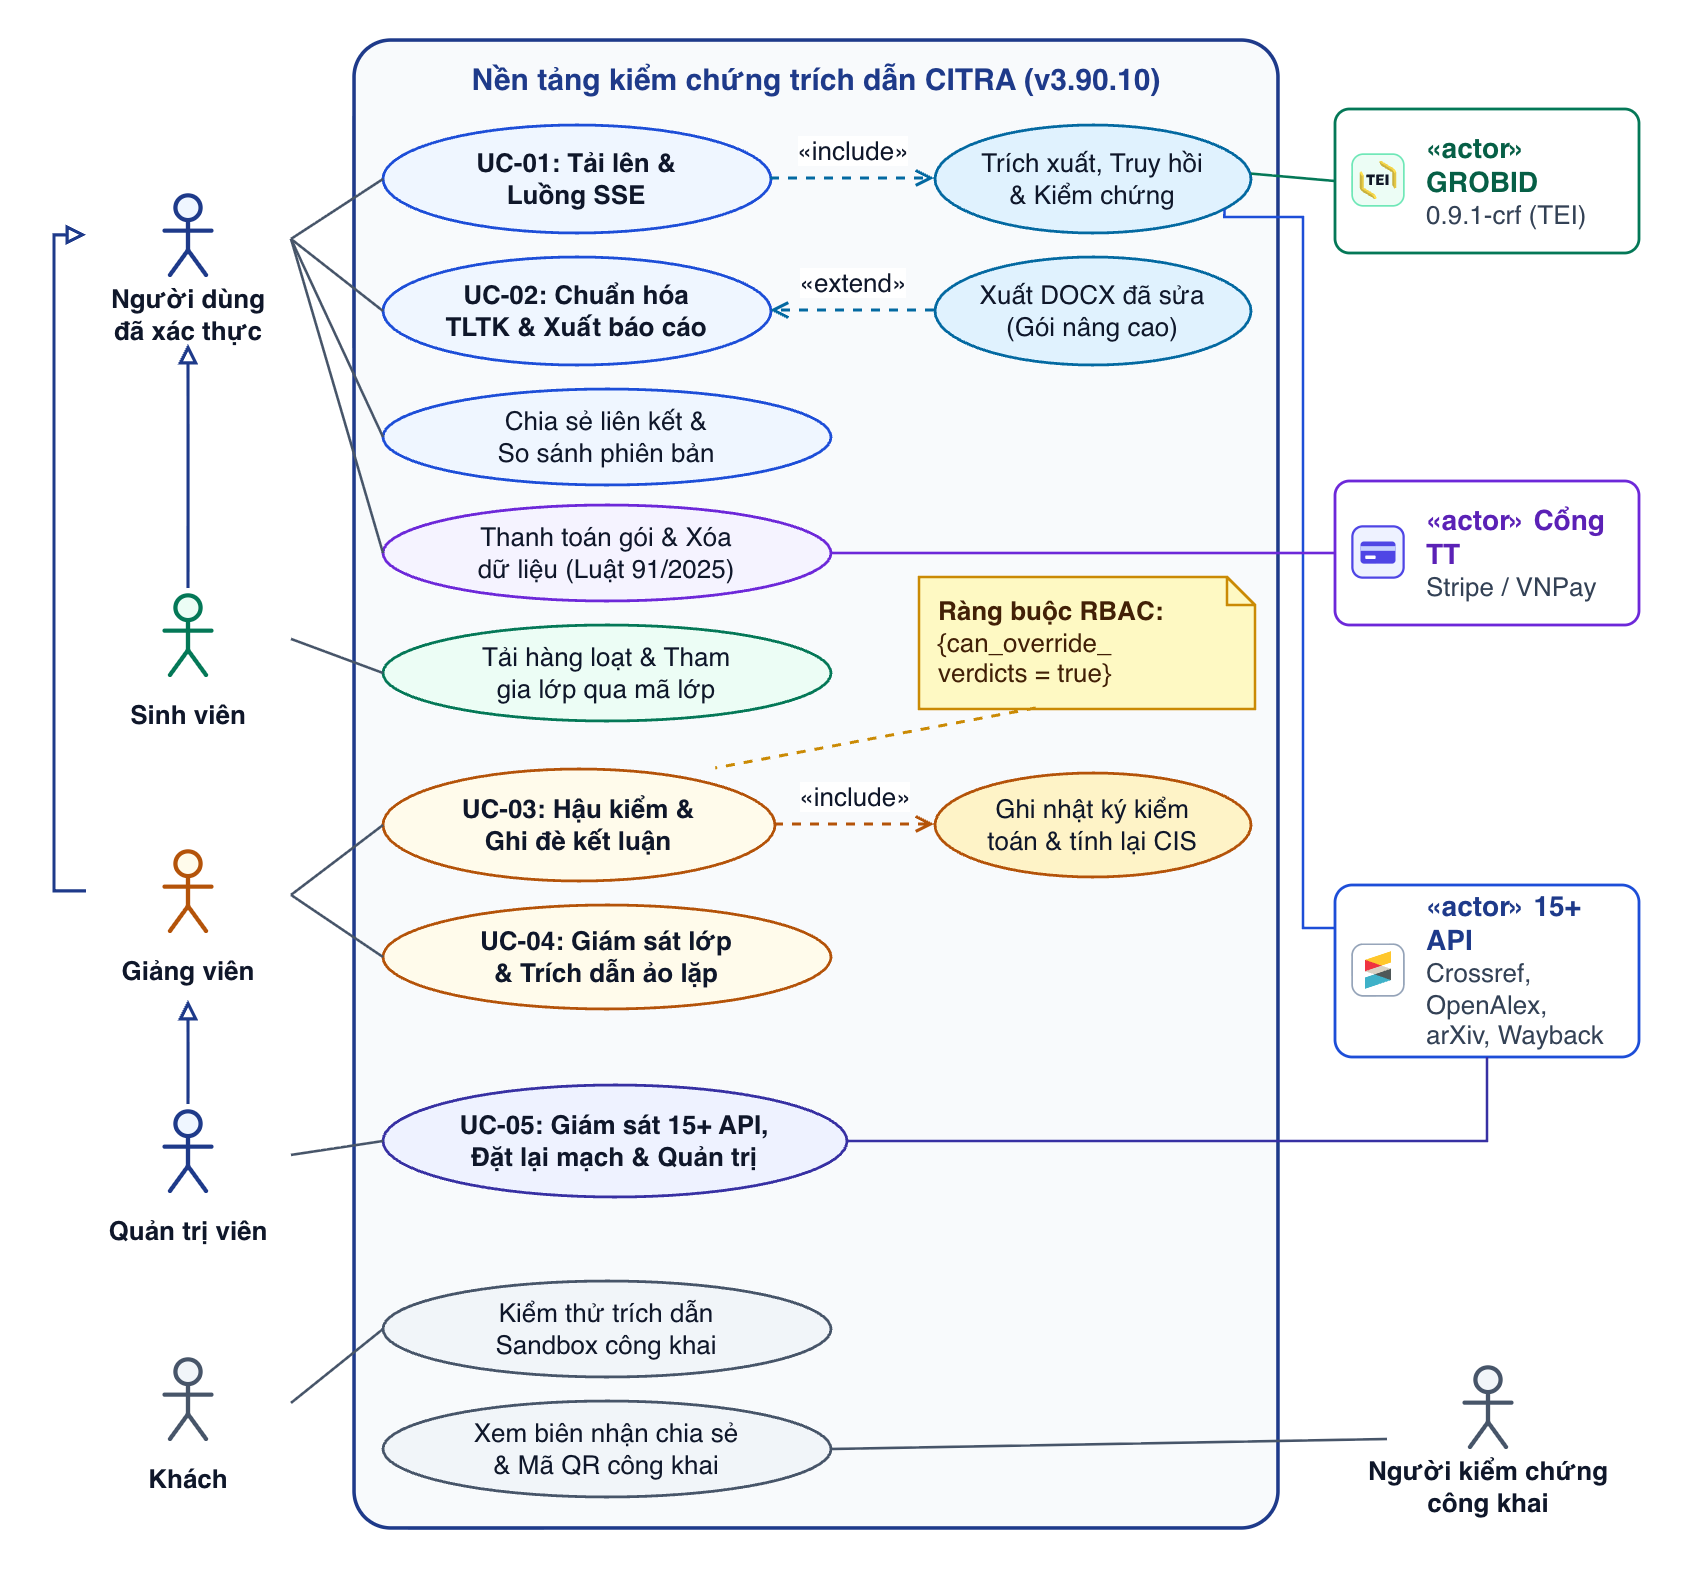
\includegraphics[width=\textwidth,keepaspectratio]{picture/figures/fig3_1_roles.png}
    \caption[Biểu đồ Ca sử dụng (Use Case) chuẩn UML 2.5 và cổng quyền hạn RBAC]{Biểu đồ Ca sử dụng (Use Case) chuẩn UML 2.5 cho ba vai trò Sinh viên, Giảng viên và Quản trị viên, làm nổi bật chốt kiểm tra quyền độc lập \texttt{\{can\_override\_verdicts = true\}}.}
    \label{fig:roles}
\end{figure}

Điểm thiết kế then chốt trong quy trình thẩm định kết luận là tách biệt tư cách vai trò khỏi thẩm quyền ghi đè thông qua cột kiểu luận lý (boolean) độc lập \texttt{users.can\_override\_verdicts}. Giảng viên phụ trách có thể cấp vai trò \texttt{teacher} cho trợ giảng để xem bài nộp của lớp và sàng lọc hàng đợi chờ duyệt, nhưng vẫn giữ \texttt{can\_override\_verdicts = False} nhằm đảm bảo chỉ giảng viên hướng dẫn chính mới có thẩm quyền đảo ngược kết luận \texttt{suspected\_hallucination}.

\subsection{Đặc tả các Ca sử dụng (Use Case) cốt lõi}

Bảng~\ref{tab:uc01}, Bảng~\ref{tab:uc02}, Bảng~\ref{tab:uc03}, Bảng~\ref{tab:uc04} và Bảng~\ref{tab:uc05} đặc tả chi tiết năm Ca sử dụng (Use Case) chính điều phối việc kiểm chứng bản thảo, sửa lỗi danh mục tài liệu tham khảo, thẩm định kết luận của giảng viên, giám sát lớp học phần và quản trị nền tảng.

\begin{longtable}{|L{0.24}|L{0.76}|}
\caption{Đặc tả Ca sử dụng (Use Case) UC-01: Tải lên bản thảo và theo dõi tiến độ kiểm chứng thời gian thực.}\label{tab:uc01}\\
\hline
\textbf{Mục đặc tả} & \textbf{Nội dung chi tiết} \\
\hline
\endfirsthead
\multicolumn{2}{c}{\itshape Bảng \thetable\ (tiếp theo trang trước)}\\
\hline
\textbf{Mục đặc tả} & \textbf{Nội dung chi tiết} \\
\hline
\endhead
\hline
\multicolumn{2}{r}{\itshape Xem tiếp trang sau}\\
\endfoot
\hline
\endlastfoot
\textbf{Mã \& Tên Ca sử dụng (Use Case)} & \textbf{UC-01:} Tải lên bản thảo và theo dõi tiến độ kiểm chứng thời gian thực (\texttt{FR-03}--\texttt{FR-12}) \\
\hline
\textbf{Tác nhân chính} & Sinh viên (\texttt{user}) hoặc Giảng viên (\texttt{teacher}) \\
\hline
\textbf{Tiền điều kiện} & Tác nhân đã đăng nhập với phiên làm việc hợp lệ và hạn mức tải lên trong tháng còn lại $\ge 1$. \\
\hline
\textbf{Hậu điều kiện} & Các bản ghi trong bảng \texttt{essays}, \texttt{citations} và \texttt{verdicts} được lưu bền vững; điểm CIS và hồ sơ chuẩn trích dẫn được lưu trữ. \\
\hline
\textbf{Luồng sự kiện chính} & \textbf{1.} Tác nhân chọn tệp \texttt{.pdf}, \texttt{.docx}, \texttt{.bib} hoặc \texttt{.ris} (tùy chọn đính kèm vào một lớp học đã ghi danh). \newline \textbf{2.} Backend kiểm tra byte định danh (magic bytes), dung lượng, giới hạn số trang và trừ hạn mức một cách nguyên tử qua cơ chế So sánh -- Hoán đổi (Compare-And-Swap -- CAS). \newline \textbf{3.} Backend lưu \texttt{EssayRecord(job\_status='queued')} và đưa tác vụ vào hàng đợi của \texttt{PipelineAdmissionController}. \newline \textbf{4.} Trình khách đăng ký luồng \texttt{GET /api/\allowbreak essays/\allowbreak\{id\}/\allowbreak events} (SSE) và hiển thị trực tiếp các giai đoạn 0--7 theo thời gian thực. \newline \textbf{5.} Tiến trình nền (worker) hoàn tất trích xuất, liên kết, truy xuất, đối sánh, kiểm tra biểu trưng/học máy và chấm điểm CIS, sau đó cập nhật \texttt{job\_status='completed'}. \newline \textbf{6.} Trình khách chuyển hướng sang trang \texttt{/verification/\allowbreak report/\allowbreak\{id\}}. \\
\hline
\textbf{Luồng rẽ nhánh / Ngoại lệ} & \textbf{2a. Sai kiểu MIME hoặc byte định danh:} Backend trả về HTTP 400; hạn mức được giữ nguyên. \newline \textbf{2b. Hết hạn mức tải lên:} Backend trả về HTTP 402/429; giao diện mở hộp thoại nâng cấp gói dịch vụ. \newline \textbf{5a. GROBID hoặc API ngoài quá thời gian chờ:} Pipeline tự động chuyển sang PyMuPDF dự phòng hoặc phát luật \texttt{R-RATE-LIMITED-ABSTAIN} (\texttt{unresolved}) mà không làm hỏng toàn bộ tác vụ. \newline \textbf{5b. Tiến trình worker gặp sự cố không thể phục hồi:} Bộ phục hồi tác vụ treo đánh dấu trạng thái \texttt{failed} và hoàn trả 1 đơn vị hạn mức qua CAS. \\
\hline
\end{longtable}

\begin{longtable}{|L{0.24}|L{0.76}|}
\caption{Đặc tả Ca sử dụng (Use Case) UC-02: Sửa lỗi danh mục tài liệu tham khảo và xuất bản thảo.}\label{tab:uc02}\\
\hline
\textbf{Mục đặc tả} & \textbf{Nội dung chi tiết} \\
\hline
\endfirsthead
\multicolumn{2}{c}{\itshape Bảng \thetable\ (tiếp theo trang trước)}\\
\hline
\textbf{Mục đặc tả} & \textbf{Nội dung chi tiết} \\
\hline
\endhead
\hline
\multicolumn{2}{r}{\itshape Xem tiếp trang sau}\\
\endfoot
\hline
\endlastfoot
\textbf{Mã \& Tên Ca sử dụng (Use Case)} & \textbf{UC-02:} Sửa lỗi danh mục tài liệu tham khảo và xuất bản thảo (\texttt{FR-13}) \\
\hline
\textbf{Tác nhân chính} & Sinh viên (\texttt{user}) hoặc Giảng viên (\texttt{teacher}) \\
\hline
\textbf{Tiền điều kiện} & Bản thảo đích thuộc quyền sở hữu của Tác nhân (hoặc thuộc lớp học do Tác nhân phụ trách) và có trạng thái \texttt{job\_status='completed'}. \\
\hline
\textbf{Hậu điều kiện} & Chuỗi danh mục tài liệu tham khảo đã định dạng chuẩn hoặc tệp \texttt{.docx} đã sửa lỗi / tệp báo cáo được tải về thành công. \\
\hline
\textbf{Luồng sự kiện chính} & \textbf{1.} Tác nhân nhấn nút \textit{Fix \& Format Citations} trên thanh tiêu đề báo cáo. \newline \textbf{2.} Backend (\texttt{GET /api/\allowbreak essays/\allowbreak\{id\}/\allowbreak remediate}) ánh xạ các trích dẫn hợp lệ và trích dẫn sai siêu dữ liệu sang các trường chuẩn từ cơ sở dữ liệu học thuật, đồng thời cô lập các mục \texttt{suspected\_hallucination} để tác giả tự xóa thủ công. \newline \textbf{3.} Tác nhân chọn chuẩn đích (\texttt{APA 7th}, \texttt{IEEE}, \texttt{TDTU}, \texttt{BibTeX} hoặc \texttt{RIS}) và xem trước bảng so sánh thay đổi từng trường. \newline \textbf{4.} Tác nhân tải xuống bản thảo \texttt{.docx} đã sửa lỗi hoặc báo cáo kiểm toán định dạng PDF/CSV/JSON đã làm sạch an toàn. \\
\hline
\textbf{Luồng rẽ nhánh / Ngoại lệ} & \textbf{2a. Trích dẫn bị nghi ngờ là trích dẫn ảo:} Hệ thống từ chối tự bịa siêu dữ liệu thay thế và gắn nhãn \texttt{hallucination} để tác giả chủ động loại bỏ. \\
\hline
\end{longtable}

\begin{longtable}{|L{0.24}|L{0.76}|}
\caption{Đặc tả Ca sử dụng (Use Case) UC-03: Thẩm định và ghi đè kết luận trích dẫn.}\label{tab:uc03}\\
\hline
\textbf{Mục đặc tả} & \textbf{Nội dung chi tiết} \\
\hline
\endfirsthead
\multicolumn{2}{c}{\itshape Bảng \thetable\ (tiếp theo trang trước)}\\
\hline
\textbf{Mục đặc tả} & \textbf{Nội dung chi tiết} \\
\hline
\endhead
\hline
\multicolumn{2}{r}{\itshape Xem tiếp trang sau}\\
\endfoot
\hline
\endlastfoot
\textbf{Mã \& Tên Ca sử dụng (Use Case)} & \textbf{UC-03:} Thẩm định và ghi đè kết luận trích dẫn (\texttt{FR-15}) \\
\hline
\textbf{Tác nhân chính} & Giảng viên (\texttt{teacher}) hoặc Quản trị viên (\texttt{admin}) có cờ \texttt{can\_override\_verdicts = True} \\
\hline
\textbf{Tiền điều kiện} & Bài nộp thuộc lớp học do Giảng viên sở hữu (hoặc Tác nhân là Quản trị viên); kết luận đích thuộc đúng bài nộp đó. \\
\hline
\textbf{Hậu điều kiện} & Nhãn kết luận được cập nhật, Điểm toàn vẹn trích dẫn (CIS) của bài nộp được tính lại và một dòng \texttt{audit\_logs} mới được chèn trong cùng một giao dịch (transaction). \\
\hline
\textbf{Luồng sự kiện chính} & \textbf{1.} Giảng viên kiểm tra một trích dẫn bị gắn cờ trong khung Chi tiết tài liệu tham khảo (Reference Inspector) hoặc hàng đợi Chờ duyệt (Pending Reviews). \newline \textbf{2.} Giảng viên chọn nhãn kết luận mới (ví dụ: \texttt{verified}) và nhập ghi chú giải trình bằng văn bản. \newline \textbf{3.} Backend (\texttt{POST /api/\allowbreak essays/\allowbreak\{id\}/\allowbreak verdicts/\allowbreak\{vid\}/\allowbreak override}) kiểm tra vai trò RBAC, cờ quyền hạn và quan hệ sở hữu giữa bài nộp với kết luận. \newline \textbf{4.} Bên trong một giao dịch cơ sở dữ liệu duy nhất, backend cập nhật \texttt{VerdictRecord}, chạy lại \texttt{CISCalculator.compute()}, cập nhật \texttt{EssayRecord.cis\_json} và chèn bản ghi \texttt{AuditLog}. \newline \textbf{5.} Giao diện làm mới vòng điểm CIS và hiển thị huy hiệu đã ghi đè. \\
\hline
\textbf{Luồng rẽ nhánh / Ngoại lệ} & \textbf{3a. Cờ quyền hạn nhận giá trị False:} Backend hủy thao tác và trả về HTTP 403 Forbidden. \newline \textbf{3b. Mã kết luận thuộc về bài nộp khác (nỗ lực tấn công IDOR):} Backend hủy thao tác và trả về HTTP 404/403. \\
\hline
\end{longtable}

\begin{longtable}{|L{0.24}|L{0.76}|}
\caption{Đặc tả Ca sử dụng (Use Case) UC-04: Giám sát lớp học phần và phát hiện bất thường chung.}\label{tab:uc04}\\
\hline
\textbf{Mục đặc tả} & \textbf{Nội dung chi tiết} \\
\hline
\endfirsthead
\multicolumn{2}{c}{\itshape Bảng \thetable\ (tiếp theo trang trước)}\\
\hline
\textbf{Mục đặc tả} & \textbf{Nội dung chi tiết} \\
\hline
\endhead
\hline
\multicolumn{2}{r}{\itshape Xem tiếp trang sau}\\
\endfoot
\hline
\endlastfoot
\textbf{Mã \& Tên Ca sử dụng (Use Case)} & \textbf{UC-04:} Giám sát lớp học phần và phát hiện bất thường chung (\texttt{FR-15}) \\
\hline
\textbf{Tác nhân chính} & Giảng viên (\texttt{teacher}) \\
\hline
\textbf{Tiền điều kiện} & Giảng viên đã đăng nhập xác thực và sở hữu ít nhất một lớp học phần. \\
\hline
\textbf{Hậu điều kiện} & Số liệu phân tích toàn lớp, các cụm trích dẫn ảo trùng lặp và bảng điểm tổng hợp định dạng ZIP/CSV được khởi tạo. \\
\hline
\textbf{Luồng sự kiện chính} & \textbf{1.} Giảng viên tạo lớp học mới và chia sẻ mã tham gia \texttt{join\_code} (định dạng mặc định \texttt{CITRA-XXXX}) cho sinh viên. \newline \textbf{2.} Sinh viên ghi danh qua \texttt{POST /api/\allowbreak teacher/\allowbreak classes/\allowbreak join} và gắn các lượt tải lên báo cáo đồ án vào lớp học. \newline \textbf{3.} Giảng viên mở trang \texttt{/teacher/\allowbreak classes/\allowbreak\{classId\}}; backend tổng hợp phân bố dải điểm CIS toàn lớp, tỷ lệ tài liệu mới trong 5 năm gần nhất, các luật bị kích hoạt nhiều nhất và những trích dẫn bịa đặt giống hệt nhau xuất hiện ở nhiều bài nộp của sinh viên. \newline \textbf{4.} Giảng viên xuất tệp tổng hợp CSV đã làm sạch hoặc gói nén ZIP chứa toàn bộ báo cáo của lớp. \\
\hline
\textbf{Luồng rẽ nhánh / Ngoại lệ} & \textbf{2a. Lộ mã tham gia lớp học:} Giảng viên tạo lại \texttt{join\_code} mới mà không làm mất danh sách sinh viên đã ghi danh trước đó. \\
\hline
\end{longtable}

\begin{longtable}{|L{0.24}|L{0.76}|}
\caption{Đặc tả Ca sử dụng (Use Case) UC-05: Giám sát viễn trắc hệ thống và đặt lại bộ ngắt mạch.}\label{tab:uc05}\\
\hline
\textbf{Mục đặc tả} & \textbf{Nội dung chi tiết} \\
\hline
\endfirsthead
\multicolumn{2}{c}{\itshape Bảng \thetable\ (tiếp theo trang trước)}\\
\hline
\textbf{Mục đặc tả} & \textbf{Nội dung chi tiết} \\
\hline
\endhead
\hline
\multicolumn{2}{r}{\itshape Xem tiếp trang sau}\\
\endfoot
\hline
\endlastfoot
\textbf{Mã \& Tên Ca sử dụng (Use Case)} & \textbf{UC-05:} Giám sát viễn trắc hệ thống và đặt lại bộ ngắt mạch (\texttt{FR-16}) \\
\hline
\textbf{Tác nhân chính} & Quản trị viên (\texttt{admin}) \\
\hline
\textbf{Tiền điều kiện} & Tác nhân đã đăng nhập xác thực với vai trò \texttt{role = 'admin'}. \\
\hline
\textbf{Hậu điều kiện} & Các bộ ngắt mạch (circuit breaker) của nhà cung cấp dữ liệu ngoài hoặc các mục bộ nhớ đệm hết hạn được đặt lại an toàn; số liệu viễn trắc được làm mới. \\
\hline
\textbf{Luồng sự kiện chính} & \textbf{1.} Quản trị viên truy cập trang \texttt{/admin/system}. \newline \textbf{2.} Backend (\texttt{GET /api/\allowbreak system/\allowbreak health}) báo cáo trạng thái sẵn sàng của GROBID, thống kê chế độ WAL của SQLite, tỷ lệ trúng bộ nhớ đệm (cache hit rate), phân bố nhãn kết luận và trạng thái bộ ngắt mạch của từng nguồn ngoài (\texttt{closed}, \texttt{half\_open}, \texttt{open}). \newline \textbf{3.} Sau khi sự cố gián đoạn của API bên ngoài đã khắc phục, Quản trị viên kích hoạt \texttt{POST /api/\allowbreak system/\allowbreak circuit-breakers/\allowbreak reset} để khôi phục lưu lượng truy vấn trực tiếp ngay lập tức. \\
\hline
\textbf{Luồng rẽ nhánh / Ngoại lệ} & \textbf{2a. Không thể kết nối container GROBID:} Bộ giám sát sức khỏe đánh dấu bộ phân tích ở trạng thái \texttt{degraded (regex fallback)} trong khi vẫn duy trì chức năng tải lên hoạt động bình thường. \\
\hline
\end{longtable}

\section{Thiết kế Quy trình Xử lý Đầu-Cuối và Xử lý Đồng thời}

\subsection{Trình tự Kiểm chứng Tám giai đoạn}

Hình~\ref{fig:workflow} trình bày biểu đồ tuần tự (Sequence Diagram) chuẩn UML 2.5 cho quy trình kiểm chứng bản thảo bất đồng bộ và thao tác thẩm định theo giao dịch của giảng viên. Khác với các đường ống yêu cầu -- phản hồi đồng bộ vốn gây nghẽn tiến trình HTTP và dễ quá thời gian chờ khi xử lý các báo cáo đồ án dài 100 trang, \textbf{CITRA} tách rời khâu tiếp nhận tệp tải lên khỏi quá trình thực thi chạy nền qua tám giai đoạn được theo dõi tường minh: (0) \texttt{parsing}, (1) \texttt{style\_detection}, (2) \texttt{extracting}, (3) \texttt{linking}, (4) \texttt{retrieving}, (5) \texttt{comparing}, (6) \texttt{checking} và (7) \texttt{scoring}. Tại ranh giới mỗi giai đoạn, bộ \texttt{ProgressTracker} an toàn luồng (thread-safe) phát các bản chụp trạng thái có cấu trúc qua giao thức Server-Sent Events (SSE) kèm cơ chế tự động thu hồi theo thời gian sống (TTL) ngay khi trình khách ngắt kết nối.

\begin{figure}[H]
    \centering
    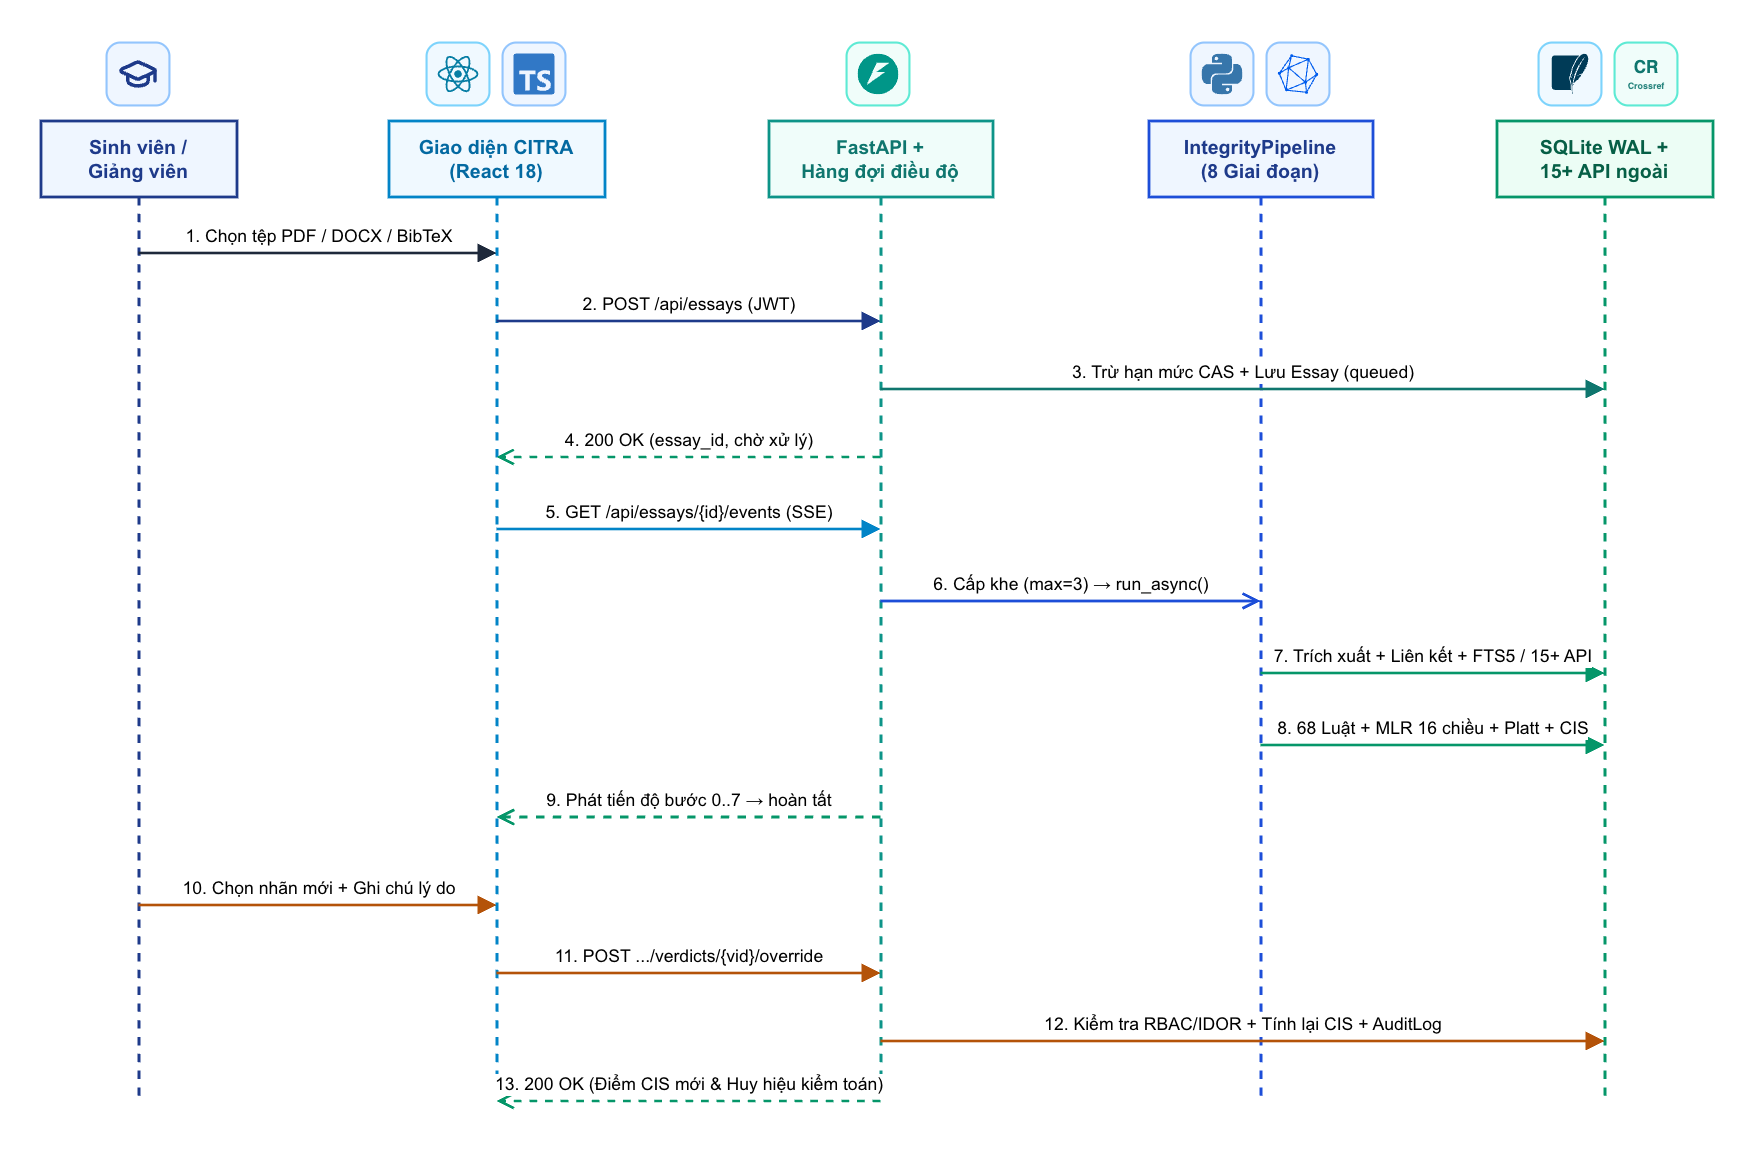
\includegraphics[width=\textwidth,keepaspectratio]{picture/figures/fig3_2_workflow.png}
    \caption[Biểu đồ tuần tự UML 2.5 cho quy trình kiểm chứng bất đồng bộ và ghi đè của giảng viên]{Biểu đồ tuần tự chuẩn UML 2.5 minh họa quy trình kiểm chứng bất đồng bộ tám giai đoạn qua SSE và giao dịch ghi đè kết luận của giảng viên.}
    \label{fig:workflow}
\end{figure}

\subsection{Kiểm soát Tiếp nhận Tác vụ, Chế độ Worker và Phục hồi Sự cố}

Vào các đợt cao điểm nộp báo cáo đồ án cuối kỳ, hàng chục sinh viên có thể tải tệp lên cùng một lúc. Việc chạy đồng thời không giới hạn các tác vụ Sentence-BERT và GROBID sẽ nhanh chóng làm cạn kiệt bộ nhớ RAM của máy chủ. \textbf{CITRA} ngăn chặn tình trạng quá tải thông qua \texttt{PipelineAdmissionController} (\texttt{api/progress.py}), điều phối cấp phát khe xử lý bằng khóa luồng (thread lock) kết hợp hàng đợi FIFO dùng \texttt{asyncio.Event} cho từng yêu cầu chờ (mặc định tối đa \texttt{max\_concurrent = 3} worker hoạt động song song), đồng thời cập nhật trực tiếp vị trí xếp hàng (\texttt{queue\_position}) tới các trình duyệt đang đợi.

Môi trường thực thi hỗ trợ ba chế độ triển khai thông qua biến cấu hình \texttt{CITRA\_WORKER\_MODE}: \texttt{inline} (gộp chung FastAPI và tiến trình xử lý nền trong một container duy nhất), \texttt{web\_only} (các nút API chỉ tiếp nhận và đẩy tác vụ vào hàng đợi trong SQLite) và \texttt{worker\_only} (tiến trình tiêu thụ nền chuyên biệt liên tục quét các tác vụ đang chờ kèm nhịp tim cập nhật \texttt{job\_heartbeat\_at} mỗi 30 giây). Để đảm bảo khả năng tự phục hồi sau sự cố sập tiến trình, mô-đun \texttt{api/job\_recovery.py} tự động rà quét các tác vụ mồ côi đang ở trạng thái \texttt{queued} hoặc \texttt{processing} ngay khi khởi động: những tác vụ bị gián đoạn có số lần thử lại nhỏ hơn \texttt{MAX\_ORPHAN\_RECOVERY\_ATTEMPTS = 2} sẽ được đưa lại vào hàng đợi một cách an toàn, trong khi các tác vụ thất bại vĩnh viễn sẽ chuyển sang trạng thái \texttt{failed} và hoàn trả nguyên tử hạn mức tải lên hằng tháng cho người dùng bằng câu lệnh SQL cập nhật theo cơ chế So sánh -- Hoán đổi (\texttt{quota\_charged: 1 $\rightarrow$ 0}), đảm bảo người dùng không bao giờ bị hoàn hạn mức hai lần hay bị trừ oan lượt tải lên.

\section{Mô hình Dữ liệu Bền vững và Kiến trúc Lưu trữ}

\subsection{Lược đồ Quan hệ và Kho Học thuật Cục bộ FTS5}

Tầng lưu trữ bền vững bao gồm \textbf{mười lăm bảng SQLAlchemy ORM} trong cơ sở dữ liệu ứng dụng chính (\texttt{data/app.db}) song hành cùng kho dữ liệu học thuật ngoại tuyến chuyên phục vụ đọc (\texttt{data/local\_papers.db}, gồm 129,137 bản ghi được đánh chỉ mục toàn văn bằng SQLite FTS5), như được tổng hợp tại Bảng~\ref{tab:data-model} và biểu diễn trực quan qua Sơ đồ Thực thể -- Kết hợp (ERD) ký hiệu chân chim (Crow's Foot) ở Hình~\ref{fig:data-model}. Các liên kết chia sẻ báo cáo công khai (\texttt{FR-14}) được cấp phát dưới dạng token phi trạng thái có chữ ký HMAC-SHA256 (\texttt{sh\_\{eid\}\_\{exp\}\_\{sig\}}) thay vì phải lưu thêm các bản ghi phiên chia sẻ khả biến trong cơ sở dữ liệu.

{\setlength{\tabcolsep}{3.5pt}
\begin{longtable}{|L{0.25}|L{0.46}|L{0.29}|}
\caption{Các thực thể SQLAlchemy ORM lưu trữ bền vững trong \texttt{db/models.py} (\texttt{v3.90.7}).}\label{tab:data-model}\\
\hline
\textbf{Tên bảng} & \textbf{Các cột chính và trách nhiệm} & \textbf{Quan hệ \& Khóa} \\
\hline
\endfirsthead
\multicolumn{3}{c}{\itshape Bảng \thetable\ (tiếp theo trang trước)}\\
\hline
\textbf{Tên bảng} & \textbf{Các cột chính và trách nhiệm} & \textbf{Quan hệ \& Khóa} \\
\hline
\endhead
\hline
\multicolumn{3}{r}{\itshape Xem tiếp trang sau}\\
\endfoot
\hline
\endlastfoot
\textbf{\texttt{users}} & Thông tin xác thực, liên kết OAuth, \texttt{role}, \texttt{can\_override\_verdicts}, \texttt{plan\_tier}, bộ đếm hạn mức, \texttt{created\_at}, \texttt{last\_login\_at} & \textbf{Quan hệ 1-N} với bài nộp, phiên, token, lớp học, ghi danh, khóa API \\
\hline
\textbf{\texttt{sessions}} & Chuỗi bearer \texttt{token} đang hoạt động, \texttt{created\_at}, \texttt{expires\_at} & \textbf{N-1} với \texttt{users}; bị thu hồi khi đăng xuất hoặc đổi mật khẩu \\
\hline
\textbf{\texttt{auth\_tokens}} & Mã băm SHA-256 dùng một lần (\texttt{token\_hash}) cho kích hoạt email và đặt lại mật khẩu & \textbf{N-1} với \texttt{users}; đánh chỉ mục trên cột \texttt{token\_hash} \\
\hline
\textbf{\texttt{api\_keys}} & \texttt{name}, \texttt{key\_prefix}, mã băm SHA-256 \texttt{key\_hash}, \texttt{created\_at}, \texttt{last\_used\_at}, \texttt{is\_active} & \textbf{N-1} với \texttt{users}; phục vụ truy cập tự động qua CLI/API \\
\hline
\textbf{\texttt{essays}} & \texttt{filename}, \texttt{num\_pages}, \texttt{job\_status}, \texttt{job\_attempt\_count}, \texttt{job\_heartbeat\_at}, \texttt{quota\_charged}, \texttt{style\_profile\_json}, \texttt{cis\_json} & \textbf{N-1} với \texttt{users} \& \texttt{classes} (tùy chọn); \textbf{1-N} với trích dẫn, kết luận \\
\hline
\textbf{\texttt{citations}} & Văn bản trích xuất (\texttt{in\_text} / \texttt{reference\_list}), các trường đã phân tích, ngữ cảnh \texttt{context}, \texttt{mapping\_status}, \texttt{citation\_link\_json} & \textbf{N-1} với \texttt{essays} (xóa dây chuyền -- cascade delete) \\
\hline
\textbf{\texttt{verdicts}} & Nhãn 5 lớp \texttt{label}, độ tin cậy đã hiệu chuẩn \texttt{confidence}, \texttt{triggered\_rules}, \texttt{mismatched\_fields}, JSON \texttt{features}, các trường ghi đè & \textbf{N-1} với \texttt{essays} (xóa dây chuyền); \textbf{1-N} với \texttt{audit\_logs} \\
\hline
\textbf{\texttt{citation\_cache}} & Khóa truy vấn đã chuẩn hóa, dữ liệu ứng viên đa nguồn đã tuần tự hóa, \texttt{hit\_count}, \texttt{created\_at}, \texttt{last\_hit\_at} & Bộ nhớ đệm toàn cục xuyên suốt các bài nộp giúp giảm gọi API lặp lại \\
\hline
\textbf{\texttt{classes}} & Tên lớp học phần, mô tả, mã tham gia duy nhất \texttt{join\_code} (\texttt{CITRA-XXXX}), \texttt{teacher\_id} & \textbf{N-1} với \texttt{users} (giảng viên); \textbf{1-N} với ghi danh \& bài nộp \\
\hline
\textbf{\texttt{class\_memberships}} & Bản ghi ghi danh sinh viên liên kết \texttt{student\_id} với \texttt{class\_id} & \textbf{Khóa tổ hợp duy nhất} \texttt{(class\_id, student\_id)} \\
\hline
\textbf{\texttt{audit\_logs}} & \texttt{verdict\_id}, tên người dùng thực hiện, \texttt{original\_label}, \texttt{new\_label}, ghi chú giải trình \texttt{note}, \texttt{logged\_at} & \textbf{N-1} với \texttt{verdicts}; không mở điểm cuối cập nhật \\
\hline
\textbf{\texttt{billing\_transactions}} & Mã phiên thanh toán, \texttt{plan\_tier}, \texttt{billing\_cycle}, số tiền USD/VND, siêu dữ liệu Stripe / VNPay, \texttt{status} & \textbf{N-1} với \texttt{users}; sổ cái đối soát giao dịch thanh toán \\
\hline
\textbf{\texttt{promo\_codes}} & Chuỗi mã giảm giá, mức giảm theo phần trăm/cố định, bộ lọc gói/chu kỳ, \texttt{max\_uses}, \texttt{used\_count}, \texttt{expires\_at} & \textbf{1-N} với \texttt{promo\_redemptions} \\
\hline
\textbf{\texttt{promo\_redemptions}} & Số tiền giảm giá đã áp dụng, \texttt{promo\_code\_id}, \texttt{user\_id}, \texttt{transaction\_id} & Bảng nối giữa \texttt{promo\_codes}, \texttt{users} và \texttt{billing\_transactions} \\
\hline
\textbf{\texttt{schema\_migrations}} & Khóa chính phiên bản \texttt{version} (\texttt{0001}--\texttt{0013}), \texttt{name}, mã kiểm tổng SHA-256 \texttt{checksum}, \texttt{execution\_ms}, \texttt{applied\_at} & Sổ cái kiểm tra tính toàn vẹn lược đồ khi khởi động \\
\hline
\end{longtable}
}

\begin{figure}[H]
    \centering
    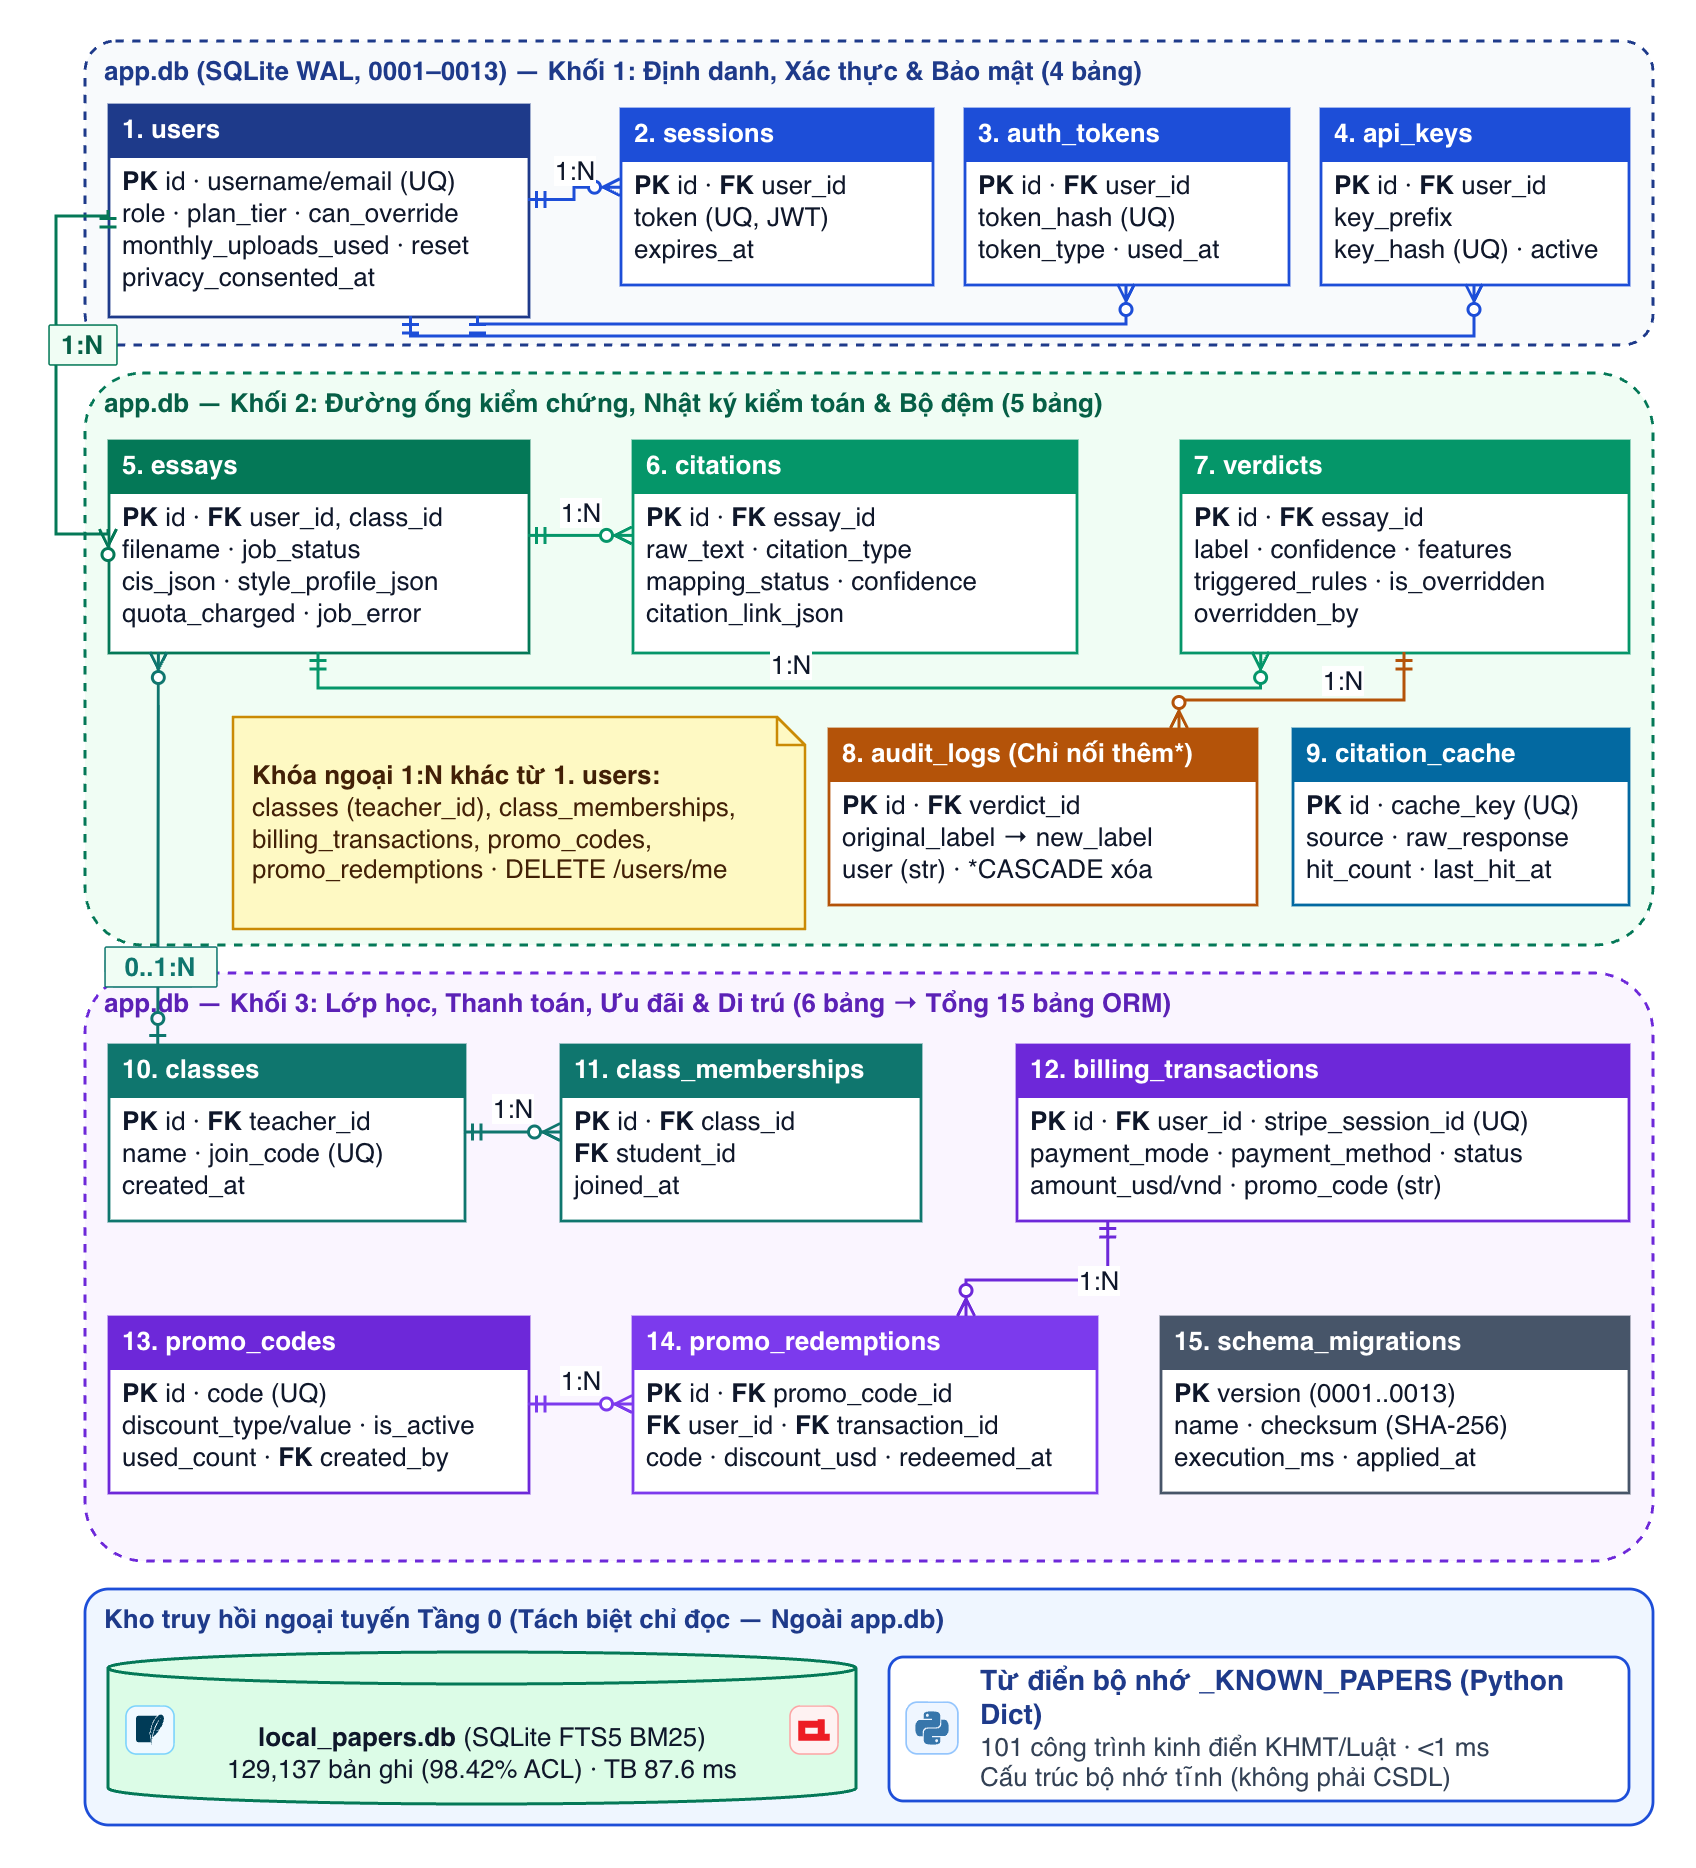
\includegraphics[width=\textwidth,keepaspectratio]{picture/figures/fig3_3_data_model.png}
    \caption[Sơ đồ Thực thể -- Kết hợp (ERD) ký hiệu chân chim của lược đồ cơ sở dữ liệu 15 bảng]{Sơ đồ Thực thể -- Kết hợp (ERD) ký hiệu chân chim của 15 bảng ORM ứng dụng (\texttt{app.db}) và kho dữ liệu học thuật ngoại tuyến SQLite FTS5 gồm 129,137 bản ghi (\texttt{local\_papers.db}).}
    \label{fig:data-model}
\end{figure}

\subsection{Di trú Lược đồ, Tinh chỉnh SQLite WAL và Lưu trữ Nhật ký Kiểm toán}

Quá trình tiến hóa lược đồ cơ sở dữ liệu qua các phiên bản được quản lý tất định bởi mô-đun \texttt{db/migrations.py}, theo dõi mười ba bản di trú đánh số thứ tự kèm mã kiểm tổng SHA-256 (\texttt{0001}--\texttt{0013}) bên trong bảng \texttt{schema\_migrations} và tự động đối chiếu mã kiểm tổng ngay lúc khởi động để phát hiện sớm mọi sai lệch lược đồ ngoài ý muốn. Để tối ưu thông lượng đọc/ghi đồng thời, \texttt{db/sqlite\_tuning.py} thiết lập \texttt{PRAGMA journal\_mode=WAL}, \texttt{synchronous=NORMAL} và \texttt{busy\_timeout=30000} trên các ổ đĩa POSIX bản địa, đồng thời tự động nhận diện phân vùng gắn kết qua macOS VirtioFS hoặc ổ đĩa mạng (nơi tệp ánh xạ bộ nhớ dùng chung \texttt{-shm} có nguy cơ gây hỏng dữ liệu) để chuyển sang chế độ nhật ký \texttt{DELETE} một cách an toàn.

Về cơ chế lưu trữ nhật ký kiểm toán, bảng \texttt{audit\_logs} không cung cấp bất kỳ điểm cuối HTTP nào cho phép sửa đổi hay xóa lẻ từng dòng trong quá trình vận hành thông thường, nhờ đó mọi thao tác ghi đè kết luận của giảng viên đều đảm bảo tính chống sửa đổi và dễ dàng đối chứng. Khi người dùng xóa một bài nộp đã tải lên hoặc thực hiện tự xóa tài khoản (\texttt{DELETE /api/users/me}), cơ chế dọn dẹp dây chuyền (cascade cleanup) sẽ xóa đồng bộ các bản ghi con trong \texttt{citations}, \texttt{verdicts} cùng các dòng \texttt{audit\_logs} liên quan bên trong một giao dịch cơ sở dữ liệu duy nhất, giúp bảo toàn tính toàn vẹn tham chiếu mà không để sót dữ liệu mồ côi.

\section{Đặc tả Giao diện API, Triển khai và Thiết kế Bảo mật}

\subsection{Bề mặt Giao diện REST và SSE API}

Toàn bộ điểm cuối (endpoint) phía máy chủ được gắn dưới tiền tố \texttt{/api} trong tệp \texttt{api/\allowbreak main.py}~\cite{fastapi}, như được trình bày chi tiết tại Bảng~\ref{tab:api-surface}. Các thao tác truy xuất SQLite và hệ thống tệp đồng bộ được đưa vào bộ thực thi vùng luồng (thread-pool executor) nhằm đảm bảo vòng lặp sự kiện \texttt{asyncio} chính không bao giờ làm nghẽn các luồng phát SSE đang hoạt động.

{\setlength{\tabcolsep}{3.5pt}
\begin{longtable}{|L{0.31}|L{0.69}|}
\caption{Các nhóm điểm cuối REST và SSE của FastAPI được gắn dưới tiền tố \texttt{/api} (\texttt{v3.90.7}).}\label{tab:api-surface}\\
\hline
\textbf{Tiền tố đường dẫn} & \textbf{Các điểm cuối và thao tác chính} \\
\hline
\endfirsthead
\multicolumn{2}{c}{\itshape Bảng \thetable\ (tiếp theo trang trước)}\\
\hline
\textbf{Tiền tố đường dẫn} & \textbf{Các điểm cuối và thao tác chính} \\
\hline
\endhead
\hline
\multicolumn{2}{r}{\itshape Xem tiếp trang sau}\\
\endfoot
\hline
\endlastfoot
\textbf{\texttt{/api/auth/*}} & \texttt{POST /register}, \texttt{/login}, \texttt{/google} \textbf{(OAuth2)}, \texttt{/logout}, \texttt{/activate}, \texttt{/forgot-password}, \texttt{/reset-password}, \texttt{GET /me}. \\
\hline
\textbf{\texttt{/api/essays/*}} & \texttt{POST /essays} (tải lên), \texttt{GET /essays}, \texttt{/essays/stats}, \texttt{/essays/\allowbreak\{id\}/\allowbreak status}, \texttt{/essays/\allowbreak\{id\}/\allowbreak events} \textbf{(SSE)}, \texttt{/essays/\allowbreak\{id\}/\allowbreak report} (\texttt{json|csv|pdf|docx}), \texttt{/essays/\allowbreak\{id\}/\allowbreak remediate}, \texttt{/essays/\allowbreak\{id\}/\allowbreak export-healed-docx}, \texttt{/essays/\allowbreak\{id\}/\allowbreak revision-diff}, \texttt{/essays/\allowbreak\{id\}/\allowbreak page-preview/\allowbreak\{p\}}, \texttt{POST /essays/\allowbreak\{id\}/\allowbreak share}, \texttt{GET /essays/\allowbreak shared/\allowbreak\{token\}}, \texttt{/essays/\allowbreak sandbox/*}. \\
\hline
\texttt{/api/essays/\allowbreak\{id\}/\allowbreak verdicts/*} & \texttt{POST /api/essays/\allowbreak\{id\}/\allowbreak verdicts/\allowbreak\{vid\}/override} (ghi đè kết luận của giảng viên có kiểm tra cờ quyền hạn + tính lại điểm CIS theo giao dịch). \\
\hline
\textbf{\texttt{/api/teacher/*}} & \texttt{GET /dashboard}, \texttt{/classes}, \texttt{POST /classes/join}, \texttt{/classes/\allowbreak\{id\}/\allowbreak regenerate-code}, \texttt{GET /classes/\allowbreak\{id\}/\allowbreak analytics}, \texttt{/classes/\allowbreak\{id\}/\allowbreak pending-reviews}, \texttt{/classes/\allowbreak\{id\}/\allowbreak export.csv}, \texttt{/classes/\allowbreak\{id\}/\allowbreak export.zip}. \\
\hline
\textbf{\texttt{/api/users/*}} & Quản trị người dùng \texttt{/users}; tự phục vụ cá nhân \texttt{PATCH/DELETE /users/me}, \texttt{/users/\allowbreak me/\allowbreak password}, \texttt{/users/\allowbreak me/\allowbreak avatar} và \texttt{/users/\allowbreak me/\allowbreak api-keys}. \\
\hline
\textbf{\texttt{/api/billing/*}} & \texttt{GET /plans}, \texttt{/subscription}, \texttt{POST /create-checkout-session}, xác thực chữ ký \textbf{HMAC-SHA512} cho Stripe \& VNPay, \texttt{/cancel} và quản trị mã giảm giá \texttt{/admin/promos}. \\
\hline
\textbf{\texttt{/api/system/*}}, \textbf{\texttt{/api/audit/*}}, \textbf{\texttt{/api/cache}}, \textbf{\texttt{/api/export/*}} & \texttt{GET /api/health}, \texttt{GET /api/\allowbreak system/\allowbreak health}, \texttt{POST /api/\allowbreak system/\allowbreak circuit-breakers/\allowbreak reset}, \texttt{DELETE /api/cache}, \texttt{GET /api/\allowbreak audit/\allowbreak log}, \texttt{GET /api/\allowbreak export/\allowbreak report} (báo cáo tổng hợp hệ thống cho quản trị viên). \\
\hline
\end{longtable}
}

\subsection{Cấu trúc Triển khai Container và Bảo mật Phòng thủ Chiều sâu}

Hình~\ref{fig:deployment} mô tả cấu trúc triển khai (Deployment Topology) chuẩn UML 2.5 trên cả môi trường phát triển (\texttt{docker-compose.yml}) lẫn môi trường vận hành thực tế đã gia cố bảo mật (\texttt{docker-compose.prod.yml}). Ba container giao tiếp qua mạng cầu nối (bridge network) Docker cô lập: \texttt{essay-\allowbreak check-\allowbreak grobid} chạy ảnh \texttt{grobid/grobid:0.9.1-crf} (được lựa chọn thay cho các ảnh học sâu nặng nề nhằm đảm bảo khâu phân tích cấu trúc PDF vận hành tất định trong vùng nhớ heap JVM 2--3\,GB trên máy chủ chỉ có CPU). Song song đó, \texttt{integrity-api} khởi chạy dịch vụ Uvicorn/FastAPI, còn \texttt{integrity-web} phân phối ứng dụng trang đơn (SPA) đã biên dịch thông qua Nginx 1.27 tích hợp TLS 1.2/1.3, tiêu đề Content-Security-Policy, HTTP Strict-Transport-Security và cơ chế chuyển tiếp luồng SSE không đệm (\texttt{X-Accel-Buffering: no}). Ở môi trường thực tế, cổng \texttt{8000} và \texttt{8070} chỉ gắn chặt vào giao diện mạng nội bộ/loopback thay vì mở trực tiếp ra Internet công cộng.

\begin{figure}[H]
    \centering
    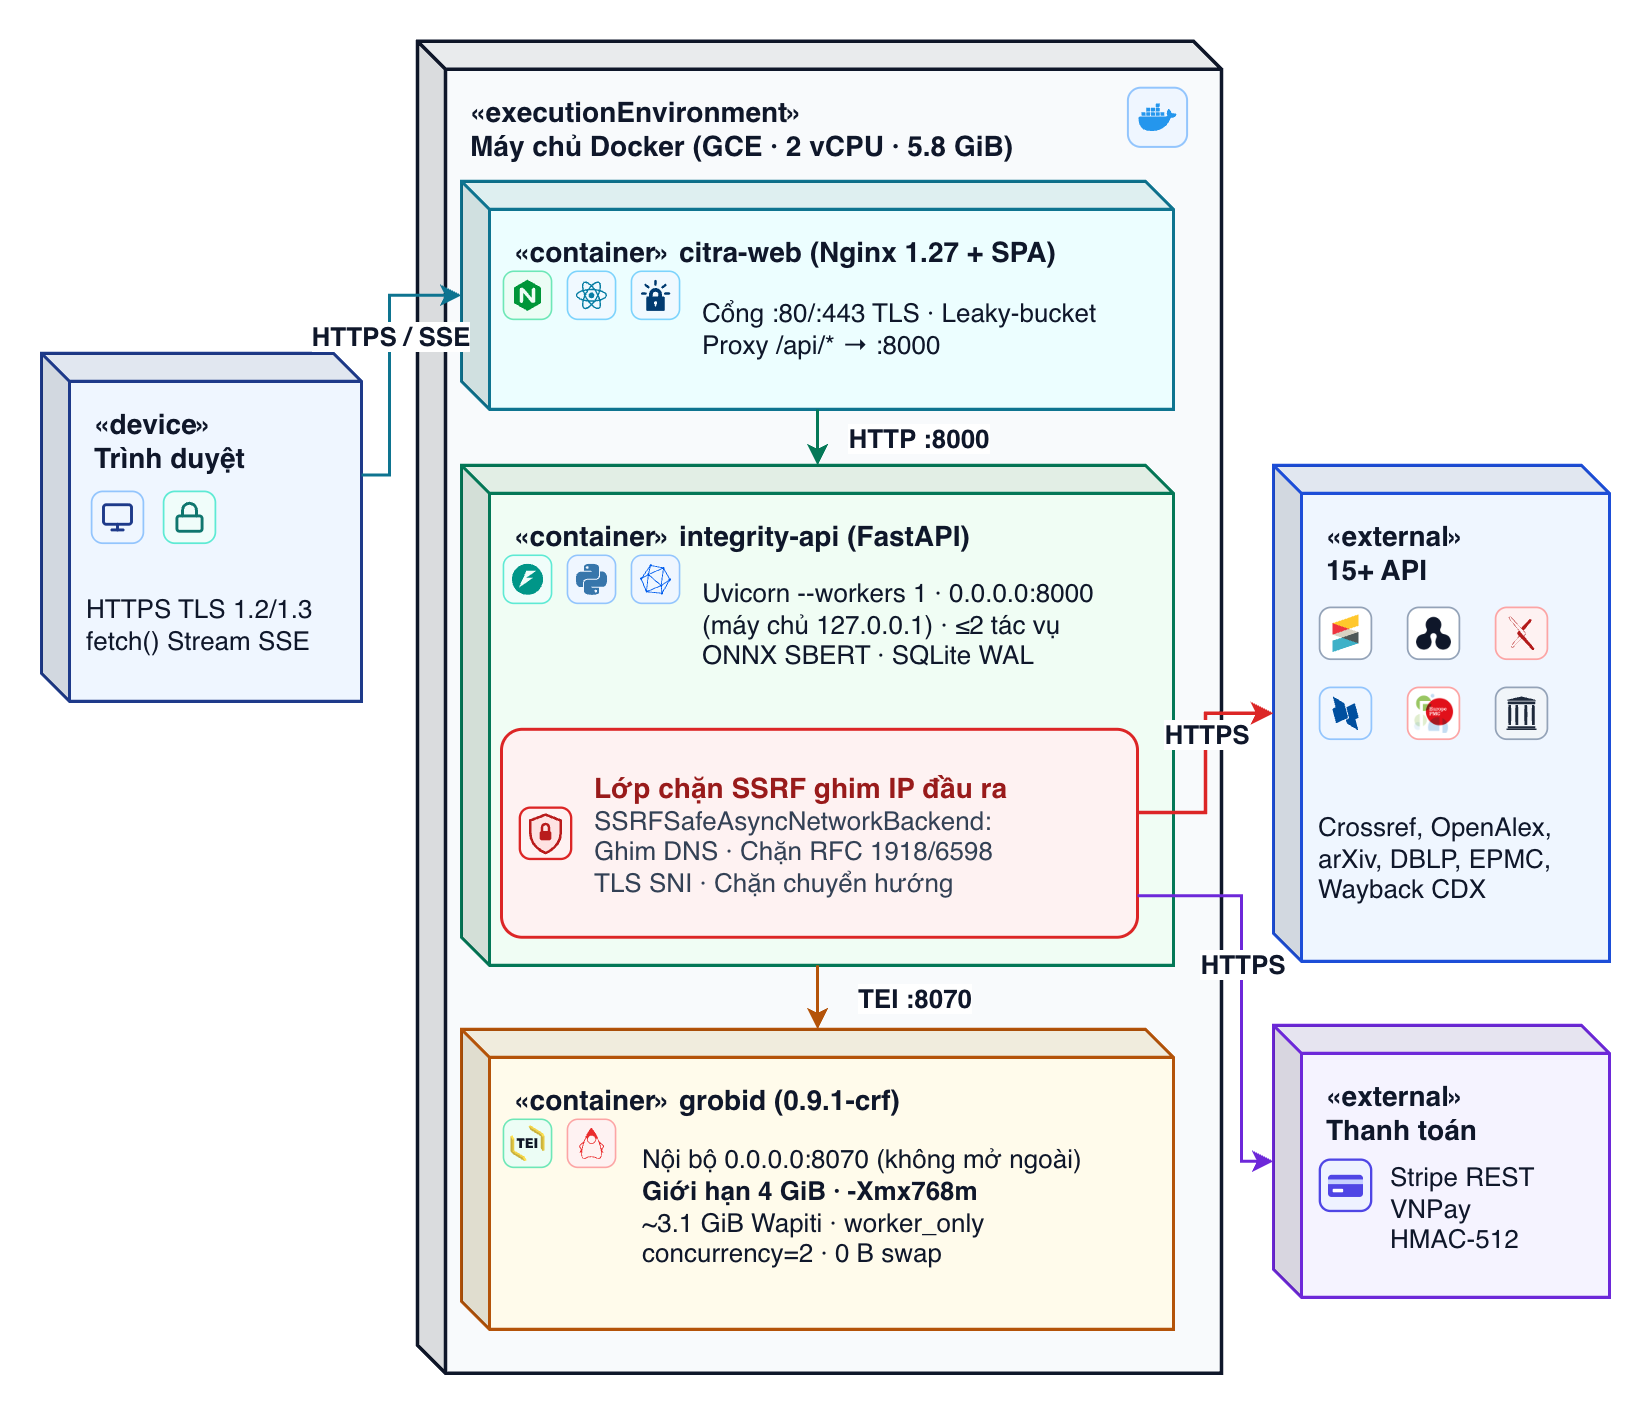
\includegraphics[width=\textwidth,keepaspectratio]{picture/figures/fig3_4_deployment.png}
    \caption[Biểu đồ triển khai UML 2.5 của nền tảng CITRA ba container]{Cấu trúc triển khai chuẩn UML 2.5 phối hợp Nginx (\texttt{integrity-web}), FastAPI (\texttt{integrity-api}) và \texttt{grobid:0.9.1-crf} tối ưu cho CPU cùng các phân vùng lưu trữ SQLite bền vững.}
    \label{fig:deployment}
\end{figure}

Các chốt kiểm soát bảo mật phòng thủ chiều sâu (defense-in-depth) bao phủ bốn lớp ranh giới:
\begin{itemize}
    \item \textbf{Gia cố Token và Thông tin xác thực:} Mật khẩu được băm bằng thuật toán \texttt{bcrypt} có trộn muối (salt); các token email dùng một lần (\texttt{auth\_tokens.token\_hash}) và khóa API cá nhân (\texttt{api\_keys.key\_hash}) chỉ lưu giá trị băm SHA-256 trong SQLite, trong khi biên nhận chia sẻ công khai sử dụng chữ ký HMAC-SHA256 phi trạng thái. Quá trình khởi động ở môi trường thực tế sẽ tự động dừng khẩn cấp nếu biến \texttt{JWT\_SECRET} vẫn giữ giá trị mặc định dùng cho phát triển.
    \item \textbf{Chống tấn công SSRF bằng kỹ thuật Ghim IP (Pinned-IP):} Hai mô-đun \texttt{LinkValidator} và \texttt{SafeHtml\allowbreak Meta\allowbreak Verifier} phân giải tên miền trước khi mở kết nối, chặn toàn bộ dải IP loopback, link-local, mạng riêng theo RFC 1918 và dịch vụ siêu dữ liệu đám mây (\texttt{169.254.\allowbreak 169.254}), kiểm tra lại từng bước chuyển hướng HTTP (redirect hop) và kết nối qua tầng truyền tải \texttt{httpx} tùy biến ghim cứng vào địa chỉ IP đã xác minh nhằm vô hiệu hóa kỹ thuật tấn công DNS rebinding.
    \item \textbf{Làm sạch Dữ liệu Tải lên và Tệp Xuất bản:} Khâu tải lên đối chiếu byte định danh của PDF (\texttt{\%PDF-}) và ZIP/DOCX (\texttt{PK\textbackslash x03\textbackslash x04}), áp đặt ngưỡng giới hạn dung lượng byte và số trang nghiêm ngặt, đồng thời vô hiệu hóa các ký tự tiền tố công thức bảng tính (\texttt{=}, \texttt{+}, \texttt{-}, \texttt{@}) khi xuất tệp CSV.
    \item \textbf{Chốt Chống IDOR và Giới hạn Tần suất Truy cập:} Mọi điểm cuối thao tác trên bài nộp, kết luận, token chia sẻ và lớp học đều kiểm tra tường minh quyền sở hữu tài nguyên (\texttt{user\_id} hoặc \texttt{class\_id} do giảng viên phụ trách) trước khi trả dữ liệu, trong khi các điểm cuối xác thực và tải lên áp dụng bộ giới hạn tần suất theo thuật toán thùng thẻ bài (token-bucket) kết hợp kế toán hạn mức nguyên tử bằng cơ chế So sánh -- Hoán đổi (\texttt{CAS}).
\end{itemize}

\section{Tóm tắt Chương}

Chương này đã đặc tả mười sáu yêu cầu chức năng nguyên tử (theo chuẩn IEEE 29148), mười yêu cầu phi chức năng định lượng (theo chuẩn ISO/IEC 25010), hệ thống mô hình Ca sử dụng (Use Case) và biểu đồ tuần tự chuẩn UML 2.5, lược đồ cơ sở dữ liệu SQLAlchemy gồm 15 bảng kèm mười ba bản di trú có kiểm tổng SHA-256 (\texttt{0001}--\texttt{0013}), hợp đồng giao diện REST/SSE dưới tiền tố \texttt{/api/*} cùng cấu trúc triển khai Docker gia cố bảo mật. Chương~\ref{chap:architecture} tiếp theo sẽ trình bày chi tiết kiến trúc phần mềm bên trong và các thuật toán xử lý xuyên suốt toàn bộ tám tầng của đường ống kiểm chứng.
